\documentclass[11pt, a4paper, spanish]{article}
\usepackage{etex}

\usepackage[a4paper, margin=2.5cm, top=3.5cm, bottom=3.5cm]{geometry} % Define los márgenes
\usepackage{amsmath, amscd, amssymb, amsthm, latexsym, gensymb} % Paquetes matemáticos
\usepackage[spanish]{babel} % Traduce los paquetes a español
\usepackage[utf8]{inputenc} % Codificación UTF8
\usepackage{fancyhdr} % Encabezados y pies de página
  \pagestyle{fancyplain}
\usepackage{enumitem}
\usepackage{xspace}
\usepackage[page, toc]{appendix} % Apéndices
\usepackage[nottoc]{tocbibind} % Referencias en la TDC
\usepackage{scrextend} % Para usar addmargin
\usepackage{listings} % Código
  \lstdefinestyle{customcpp}{
    belowcaptionskip=1\baselineskip,
    breaklines=true,
    xleftmargin=3em,
    language=C++,
    basicstyle=\small\ttfamily
  }
\usepackage[onelanguage, spanish]{algorithm2e}
  % \NoCaptionOfAlgo
  \LinesNumbered\RestyleAlgo{ruled}\IncMargin{1em}\DontPrintSemicolon\SetArgSty{}\SetCommentSty{textsf}\SetFuncSty{textsf}
  \SetKwProg{For}{para}{ hacer}{fin}
  \SetKwProg{Fn}{función}{:}{fin}
\usepackage[pdftex]{graphicx} % Imágenes
\usepackage[usenames,dvipsnames]{color} % Autoexplicativo
% \usepackage{caption} % Captions sin números
% \usepackage{multirow} % Celdas multifila en tablas
\usepackage[thinlines]{easytable} % Tablas para diagramas de registros
\usepackage{tabu} % Tablas para diagramas de registros
\usepackage{caratula} % Carátula del DC

% Bibliografía
% \usepackage{biblatex}
% \addbibresource{referencias.bib}

% Comandos personalizados
\let\strong\textbf
\renewcommand{\appendixtocname}{Apéndices}
\renewcommand{\appendixpagename}{Apéndices}
\theoremstyle{plain}
  \newtheorem{prop}{Proposición}
  \newtheorem{lema}{Lema}
\theoremstyle{remark}
  \newtheorem{obs}{Observación}
\setlength{\parskip}{.3em}
\newcommand{\acr}[1]{\textsc{\lowercase{#1}}} % Acrónimos
\newcommand{\mat}[1]{\ensuremath{\mathbf{#1}}}
\newcommand{\img}[1]{\mat{#1}}
\newcommand{\comp}[1]{\ensuremath{\mathsf{#1}}}

\newenvironment{bitlimits}[2]{caca}{caca}

% Encabezado
\lhead{Organización del Computador II}
\rhead{Trabajo Práctico Nº 2}
% Pie de pagina
\renewcommand{\footrulewidth}{0.4pt}
% \lfoot{FCEN}
% \rfoot{UBA}

\begin{document}

% Datos de carátula
\materia{Organización del Computador II}
\titulo{Trabajo Práctico Nº 2}
\fecha{Segundo cuatrimestre de 2015}
\grupo{Grupo: Smelly Cat}

\integrante{Frizzo, Franco}{013/14}{francofrizzo@gmail.com}
\integrante{Martínez, Manuela}{160/14}{martinez.manuela.22@gmail.com}
\integrante{Rabinowicz, Lucía}{105/14}{lu.rabinowicz@gmail.com}

% Carátula
\maketitle
\newpage

% Índice
\tableofcontents
\clearpage

% Contenido
\section{Introducción}

  En el presente trabajo, aplicamos el modelo de programación vectorial \acr{SIMD} (\emph{Single Instruction, Multiple Data}) para la implementación de filtros para el procesamiento de imágenes. Más precisamente, llevamos a cabo la implementación de los siguientes dos filtros:
  \begin{itemize}
    \item \emph{Diferencia}, que recibe como entrada dos imágenes y devuelve como resultado otra imagen que indica dónde difieren las dos primeras.
    \item \emph{Blur gaussiano}, que suaviza la imagen reemplazando cada píxel por un promedio de los píxeles circundantes, ponderado según una función gaussiana.
  \end{itemize}

  La elaboración del trabajo se dividió en dos etapas. En primer lugar, implementamos ambos filtros tanto en lenguaje C como en lenguaje ensamblador para la arquitectura x86 de Intel. En este último caso, se utilizaron las instrucciones \acr{SSE} de dicha arquitectura, que aprovechan el ya mencionado modelo \acr{SIMD} para procesar datos en forma paralela.

  Una vez realizadas estas implementaciones, las sometimos a un proceso de comparación para extraer conclusiones acerca de su rendimiento. Con este fin, experimentamos con variaciones tanto en los datos de entrada como en detalles implementativos de los mismos algoritmos. De esta manera pudimos recopilar datos sobre el comportamiento de cada implementación, y contrastar estos resultados con diversas hipótesis previamente elaboradas.

\section{Desarrollo}

  \subsection{Consideraciones generales}
    Las imagenes que se utilizan como entrada y salida de los algoritmos a implementar son matrices de píxeles. Cada uno de estos píxeles está representado por cuatro enteros sin signo de 8 bits de profundidad (es decir, en el rango [0, 256)), que contienen, respectivamente, los valores de los colores azul (\textsf{b}), verde (\textsf{g}) y rojo (\textsf{r}), y la transparencia (\textsf{a}).

    Se usará la notación $\img{I}_{x,y}$ para referirse al píxel ubicado en la fila $x$ y la columna $y$ de la imagen $\mat{I}$, y la notación $\mat{I}_{x,y}^k$ para hacer referencia al valor de la componente $k$ de este píxel, donde $k \in \lbrace \comp{b, g, r, a} \rbrace$.
  
  \subsection{Diferencia de imágenes}
    Este filtro recibe dos imágenes como entrada y devuelve como salida una tercera imagen que muestra, en cada píxel, la diferencia entre los píxeles correspondientes de las imágenes de entrada, ignorando la componente \textsf{a}. Más especificamente, si $\img{I_1}$ e $\img{I_2}$ son las imágenes de entrada y $\img{O}$ es la imagen de salida, entonces:

    \[ \img{O}_{x,y}^k = \begin{cases}
      \displaystyle \max_{k \in \lbrace \comp{b, g, r} \rbrace} \left( \left\vert {\img{I_1}}_{x,y}^k - {\img{I_2}}_{x,y}^k \right\vert \right)
        & \text{si } k \in \lbrace \comp{b, g, r} \rbrace \\
      255
        & \text{si } k = \comp{a}
    \end{cases} \]

    \subsubsection{Implementación en lenguaje C}
      La implementación de este filtro en lenguaje C es sumamente sencilla. Ambas imágenes de entrada se recorren simultáneamente mediante dos ciclos anidados, que iteran sobre sus filas y sus columnas, respectivamente. Para las componentes \textsf{b}, \textsf{g} y \textsf{r} de cada píxel, se calcula el valor absoluto de la diferencia entre los valores correspondientes a ambas imágenes. Luego, se computa el máximo entre estos tres valores, que se guarda como el valor de las componentes \textsf{b}, \textsf{g} y \textsf{r} para el píxel correspondiente en la imagen de salida. Por último, la componente \textsf{a} de dicho píxel se define como 255.

    \subsubsection{Implementación en lenguaje ensamblador}
      Al implementar el filtro en lenguaje ensamblador, es posible aprovechar las ventajas que brinda el modelo \acr{SIMD}. En particular, dado que los registros \texttt{XMM} son de 16 bytes, se los puede utilizar para procesar 4 píxeles de las imágenes en paralelo, reduciendo la cantidad de iteraciones del algoritmo y, particularmente, de accesos a memoria necesarios para completar el algoritmo.

      La implementación en este lenguaje del filtro consiste principalmente de un ciclo que itera sobre la imagen. Al comienzo de cada ejecución, se copian 4 píxeles de $\img{I_1}$ al registro \texttt{XMM0}, y los correspondientes 4 píxeles de $\img{I_2}$ a \texttt{XMM1}.

      \begin{center}
        \raisebox{2.5mm}{\texttt{XMM0:}} 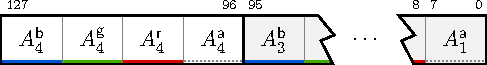
\includegraphics{imagenes/diff-registros-1.pdf}

        \raisebox{2.5mm}{\texttt{XMM1:}} 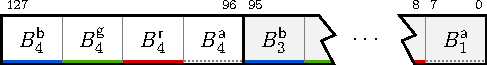
\includegraphics{imagenes/diff-registros-2.pdf}
      \end{center}

      El paso siguiente consiste en calcular, para cada una de las componentes de estos píxeles, el valor absoluto de la diferencia entre ambas imágenes. Para realizar esto, se realiza la resta de las dos maneras posibles, obtenie $\mathtt{XMM0} = \mathtt{XMM0} - \mathtt{XMM1}$ y $\mathtt{XMM1} = \mathtt{XMM1} - \mathtt{XMM0}$. En las posiciones donde el valor contenido en \texttt{XMM0} sea mayor que el de \texttt{XMM1}, será válido el resultado de la primera operación, mientras que en las demás posiciones se deberá tener en cuenta el segundo resultado.

      Para seleccionar cuál de los dos resultados es el correcto, se utiliza una máscara que se obtiene comparando los valores de \texttt{XMM0} y \texttt{XMM1}. Aquí aparece un problema, ya que debemos comparar enteros sin signo, y \acr{SSE} no brinda instrucciones para hacer esto. Es por eso que se recurre a desempaquetar los números y considerarlos como enteros con signo de dos bytes, que sí se pueden comparar. Empaquetando luego el resultado obtenido, se logra la máscara buscada. Esta se aplica mediante \texttt{PAND} al valor contenido en \texttt{XMM0} y mediante \texttt{PANDN} al valor presente en \texttt{XMM1}. Posteriormente se computa un \texttt{POR} entre los valores recién calculados, llegando al valor deseado, que se almacena en \texttt{XMM0}.

      Por último, es necesario calcular la norma infinito de las componentes \textsf{b}, \textsf{g} y \textsf{r} obtenidas. Para hacer esto, se copia en \texttt{XMM1} el último resultado y se lo desplaza un byte hacia la izquierda.

      \begin{center}
        \raisebox{2.5mm}{\texttt{XMM0:}} 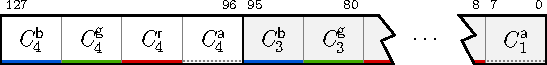
\includegraphics{imagenes/diff-registros-3.pdf}

        \raisebox{2.5mm}{\texttt{XMM1:}} 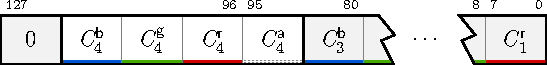
\includegraphics{imagenes/diff-registros-4.pdf}
      \end{center}

      A continuación puede usarse la instrucción \texttt{PMAXUB XMM1, XMM0} para calcular el máximo entre estos dos registros, obteniendo 

      \begin{center}
        \raisebox{2.5mm}{\texttt{XMM1:}} 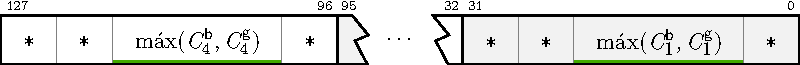
\includegraphics{imagenes/diff-registros-5.pdf}
      \end{center}

      Repitiendo el proceso anterior, pero esta vez almacenando el resultado en \texttt{XMM0}, se obtiene

      \begin{center}
        \raisebox{2.5mm}{\texttt{XMM0:}} 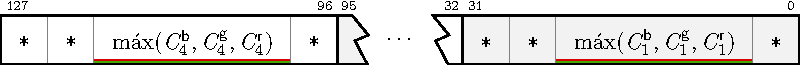
\includegraphics{imagenes/diff-registros-6.pdf}
      \end{center}

      A partir de aquí, utilizando la instrucción \texttt{PSHUFB} para replicar el valor calculado, se almacena este máximo en las componentes \textsf{r}, \textsf{g} y \textsf{b} de los píxeles correspondientes de la imagen de destino, y utilizando una máscara adecuada, se define la componente \textsf{a} de todos ellos como 255.

  \subsection{Blur gaussiano}
    Este filtro recibe una imagen como entrada y devuelve como salida el resultado de aplicarle una convolución\footnote{Dadas dos funciones $f$ y $g$, una \emph{convolución} $f * g$ es una operación que las transforma en una tercera función: $(f * g)(t) = \int_{-\infty}^{+\infty} f(\tau) g(t - \tau) \,d\tau$ en el caso continuo, $(f * g)_n = \sum_{k=-\infty}^{+\infty} f_k g_{n-k}$ ($n, k \in \mathbb{Z}$) en el caso discreto.} con una función gaussiana, que dependerá de un parámetro $\sigma$ que podrá ser modificado. Dada la naturaleza del problema, trabajaremos con una convolución discreta en dos dimensiones, y como nuestro poder de cómputo es limitado, procesaremos solo una vecindad acotada de cada píxel, cuyo radio quedará determinado por un parámetro configurable $r$. En definitiva, el resultado del filtro será

    \[ \img{O}_{x,y}^k = \begin{cases}
      \displaystyle \sum_{i=-r}^r \sum_{j=-r}^r \img{I}_{x+i,y+j}^k \mat{K}_{r-i,r-j}
        & \text{si } k \in \lbrace \comp{b, g, r} \rbrace \\
      255
        & \text{si } k = \comp{a}
    \end{cases} \]

    donde $\mat{K}$ es la matriz o \emph{kernel} de la convolución, con

    \[ \mat{K}_{i,j} = \frac{1}{2 \pi \sigma^2} e^{- \frac{(r-i)^2 + (r-j)^2}{2 \sigma^2}} \qquad \text{para todo } 0 \leq i,j \leq 2r \]

    \subsubsection{Implementación en lenguaje C}

      Para aplicar el filtro, es necesario que el parámetro $r$ sea menor que la mitad de la cantidad de filas y menor que la mitad de la cantidad de columnas. Por esto, verificamos que el parámetro cumpla con estas condiciones. El siguiente paso consiste en crear la matriz de convolución del filtro llamando a una función auxiliar, explicada más adelante. 

      Luego, mediante dos ciclos, se recorre toda la parte de la imagen original a la que es posible aplicarle el filtro. Esta parte es la que contempla las filas desde el valor del radio hasta $filas - (r + 1$), y las columnas desde el valor del radio hasta $columnas - (r + 1$). El resto de la imagen no será afectada. 

        \begin{figure}
          \centering 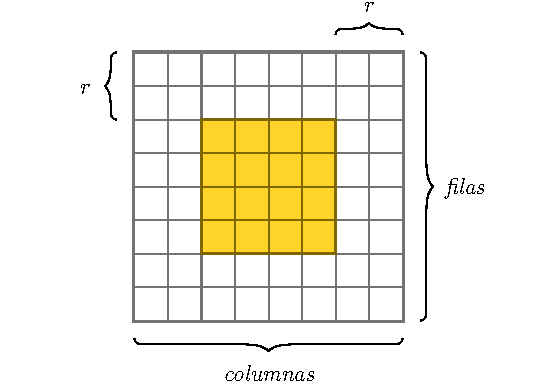
\includegraphics{imagenes/zona-afectada.pdf}
          \caption{Sector de la imagen afectado por el filtro.} \label{fig:zona-afectada}
        \end{figure}

      En cada paso de esta iteración, se llama a la función \texttt{afectarPixel}, que se ocupa de modificar cada píxel correctamente, utilizando la matriz de convolución creada anteriormente. 

      \subsubsection*{Función \texttt{matrizDeConvolucion}}

        En esta parte del algoritmo se calcula la matriz de la convolución. Para ello, en primer lugar, se piden $4 \times (2r + 1)^2$ bytes de memoria, lugar que va a ocupar la matriz ya que su altura es $2r + 1$ y su ancho, $4 \times (2r 1)$ (porque cada píxel ocupa 4 bytes).
        
        Se utilizan dos ciclos; ambos van desde 0 hasta $2r + 1$. 
        
        \begin{figure}
          \centering 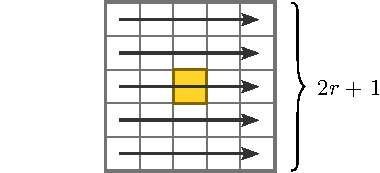
\includegraphics{imagenes/matriz-de-convolucion-c.pdf}
          \caption{Ejemplo de funcionamiento de la implementación en C de \texttt{matrizDeConvolucion} con $r = 2$.} \label{fig:matriz-de-convolucion-c}
        \end{figure}

        En cada paso, se calcula la función gaussiana con el $\sigma$, $r$, $i$ y $j$ correspondientes, donde $i$ representa la fila y $j$ la columna. Luego, se coloca el resultado en la fila $i$, columna $j$ de la matriz. Finalmente, se devuelve un puntero a la primera posición de la matriz.

      \subsubsection*{Función \texttt{afectarPixel}}
        Primero se inicializan 3 variables donde luego se van a almacenar las sumas que corresponden a cada componente del píxel a afectar (\textsf{b}, \textsf{g} y \textsf{r}). 

        Seguidamente, se utilizan dos ciclos para recorrer la matriz de convolución y la parte de la imagen correspondiente a los vecinos del píxel a afectar. 
        
        Estos van desde $0$ hasta $(2r)$, para recorrer las filas, y desde $0$ hasta $(2r \times 4)$ para recorrer las columnas. En cada paso se multiplica el valor de las componentes del píxel observado por el valor de la matriz de convolución. El resultado de esta multiplicación se suma en las 3 variables creadas en el principio. 
        
        Finalmente, se copia el valor de cada variable en cada componente del píxel en la imagen destino. Luego, en la componente \textsf{a} se coloca el valor 255.  

    \subsubsection{Implementación en lenguaje ensamblador} 
      Este algoritmo se ocupa de recorrer toda la porción de la imagen a la que es posible aplicarle el filtro. 
      
      Al igual que en la implementación en C, primero se hace una comparación para revisar si el radio es válido. 
      
      Luego, utilizando la instrucción \texttt{CALL}, se hace un llamado a la función \texttt{matrizDeConvolución} (implementada en C), la cual devuelve un puntero a la matriz de convolución creada. 
      
      Posteriormente, se utilizan dos ciclos para recorrer la porción a modificar de la imagen. Estos utilizan los registros \texttt{R8} para recorrer las columnas y \texttt{R9} para recorrer las filas.

      \begin{figure}
        \centering 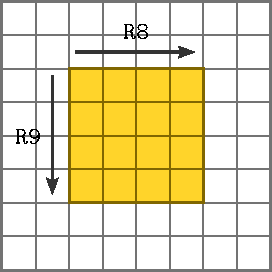
\includegraphics{imagenes/ciclos-asm.pdf}
        \caption{Aplicación del filtro en la implementación en lenguaje ensamblador, con $r = 2$.} \label{fig:ciclos-asm}
      \end{figure}

      En cada paso del ciclo, utilizando nuevamente la instrucción \texttt{CALL}, se realiza un llamado a la función afectarPixel (implementada en ensamblador) que se ocupa de modificar el píxel correspondiente. 

      \paragraph{Función \texttt{afectarPixel}}
        El primer paso de este algoritmo es encontrar el puntero al píxel que se debe afectar en la imagen original y otro puntero al mismo píxel pero en la imagen destino. Estos punteros son guardados en los registros \texttt{R12} y \texttt{R14}, respectivamente.   

        Llamaremos \emph{submatriz imagen} a la porción de la imagen original que se debe utilizar para que, junto con la matriz de convolución, se obtenga el nuevo valor del píxel. Esta submatriz es la que contiene al píxel a modificar en el centro y su tamaño es el mismo que el de la matriz de convolución. 
        
        \begin{figure}
          \centering 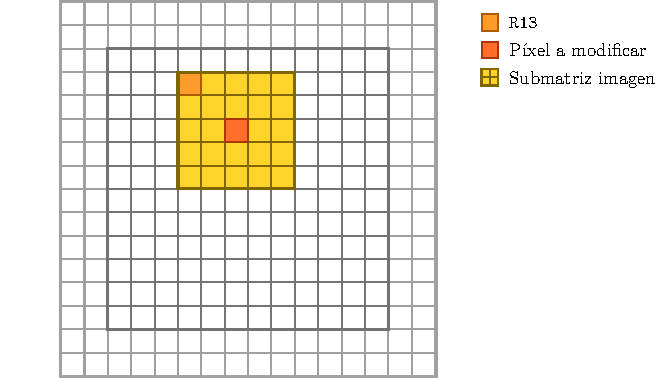
\includegraphics{imagenes/afectar-pixel-asm.pdf}
          \caption{Implementación en ensamblador de \texttt{afectarPixel} con $r = 2$.} \label{fig:afectar-pixel-asm}
        \end{figure}

        Luego, se debe encontrar el puntero al primer píxel de la submatriz imagen. Esto se calcula de la siguiente manera: $\mathtt{R12} - 4 \times (r - r \times columnas)$. Este puntero se encuentra en el registro r13 y es utilizado para recorrer la submatriz. 

        En el registro \texttt{R11} se guarda la cantidad total de píxeles que componen la submatriz imagen. 

              $\mathtt{R11} = (2 \times r + 1)^{2}$  
        
        El registro \texttt{R15} contiene el tamaño de las filas.
        
              $\mathtt{R15} = (2 \times r + 1)$

        Estos últimos dos se utilizan como registros contadores.

        A continuación, se recorren por filas la submatriz imagen y la matriz de convolución a la vez. \texttt{R11} se utiliza para saber cuando finalizar el bucle, es decir, cuando ya se observaron todos los píxeles. Estos son procesados utilizando instrucciones \acr{SSE} y registros del tipo \texttt{XMM}. En cada uno de estos registros es posible guardar 4 píxeles, ya que cada píxel ocupa 4 bytes. 

        \begin{center}
          \raisebox{2.5mm}{\texttt{XMM:}} 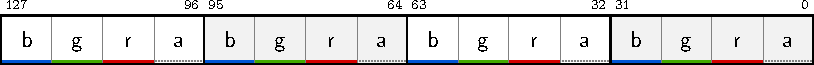
\includegraphics{imagenes/blur-registros-1.pdf}
        \end{center}
  
        En cada paso de este ciclo se considera una fila, utilizando \texttt{R15} para saber cuándo termina. Se toman 4 píxeles de la submatriz imagen y los correspondientes 4 de la matriz de convolución. Luego de desempaquetar los píxeles se realiza la multiplicación de cada componente (\textsf{b}, \textsf{g} o \textsf{r}) con el valor de la matriz de convolución que le corresponde. El resultado de cada producto se suma al registro \texttt{XMM6}. 

        \vspace{\baselineskip}

        \noindent \begin{minipage}{\textwidth}
          \begin{enumerate}
            \item Píxel desempaquetado

            {\centering \noindent \raisebox{2.5mm}{\texttt{XMM:}} 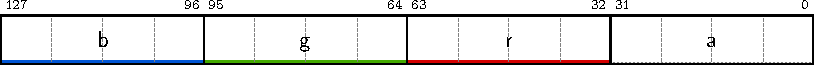
\includegraphics{imagenes/blur-registros-2.pdf}}

            \item Valor en la matriz de convolución

            {\centering \noindent \raisebox{2.5mm}{\texttt{XMM:}} 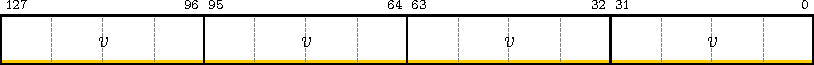
\includegraphics{imagenes/blur-registros-3.pdf}}

            \item Resultado

            {\centering \raisebox{2.5mm}{\texttt{XMM:}} 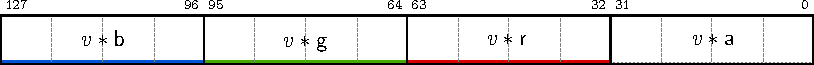
\includegraphics{imagenes/blur-registros-4.pdf}}
          \end{enumerate}
        \end{minipage}

        \vspace{\baselineskip}

        Se puede notar que el tamaño de las filas es congruente a 1 o 3 módulo 4. Por lo tanto, se procesan de a 4 píxeles hasta llegar a alguno de los dos casos borde posibles: cuando queda 1 píxel por computar o cuando quedan 3. 
        
        La solución a este problema es tomar y desempaquetar los píxeles de la submatriz imagen que todavía no fueron procesados junto con sus siguientes, hasta completar 4. Esto es así en todos los casos, excepto en el que los píxeles restantes son los últimos de la submatriz imagen (es decir, los que se corresponden con la última fila). En este caso, se toman los píxeles anteriores, ya que de otra forma, si el píxel a modificar se encontrase en alguna de las 3 últimas posiciones se accedería a posiciones de memoria fuera de la imagen. Estos píxeles no se tienen en cuenta a la hora de realizar el cálculo.

        Esto mismo se realiza para la matriz de convolución.
          
        \begin{figure}
          \centering 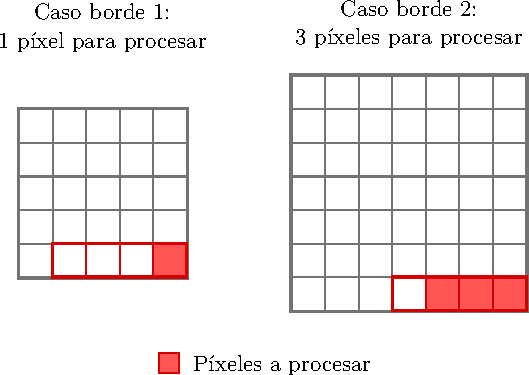
\includegraphics{imagenes/casos-borde-asm.pdf}
          \caption{Tratamiento de casos borde en la implementación en ensamblador de \texttt{afectarPixel}.} \label{fig:casos-borde-asm}
        \end{figure}

        Al finalizar el ciclo, se tiene en \texttt{XMM6} el valor esperado para cada componente (\textsf{b}, \textsf{g} y \textsf{r}) del píxel a afectar, en punto flotante de 32 bits. Primero se pasan estos valores a enteros; después, en la componente \textsf{a} se coloca un 255, y luego se empaqueta \texttt{XMM6} para copiarlo en la posición del píxel que se quiere modificar en la imagen destino.

\section{Experimentos}
	%Todos los experimentos se repitieron 20 veces. Para reproducirlos se debe ejecutar exp/exp.sh -n 20  
	
	\subsection{Experimento 1}
		En el primer experimento se genera una determinada cantidad de imágenes tomando una imagen grande y cambiando su tamaño disminuyendo sus dimensiones.
	
		Luego, se ejecuta el filtro Blur con cada una de las imágenes y se compara el tiempo de ejecución de las implementaciones en C y assembler.
	
		Esto se repite para el filtro Diff, con la diferencia de que para cada tamaño de imágen se generan dos imágenes con ciertas modificaciones para poder observar el buen funcionamiento del mismo.


	\subsubsection{Hipótesis} 
		El resultado esperado es que la implementación en assembler de ambos filtros sea más eficiente, sin importar el tamaño de la imagen. Esto sucede ya que a diferencia de C, assembler utiliza SIMD para procesar píxeles, por lo tanto es posible trabajar con 4 píxeles en simultaneo.

	\subsubsection{Valores utilizados como parámetros} 		
		En este experimento el ancho de las imágenes utilizadas como parámetro se encuentran en un rango entre 24 y 1800 píxeles.Además, para el filtro Blur se utilizó $Radio = 15$ y $Sigma = 5$.

	\subsubsection{Resultados}
   	{\centering \begin{tabular}{c}
      {\small Filtro Diferencia} \\
      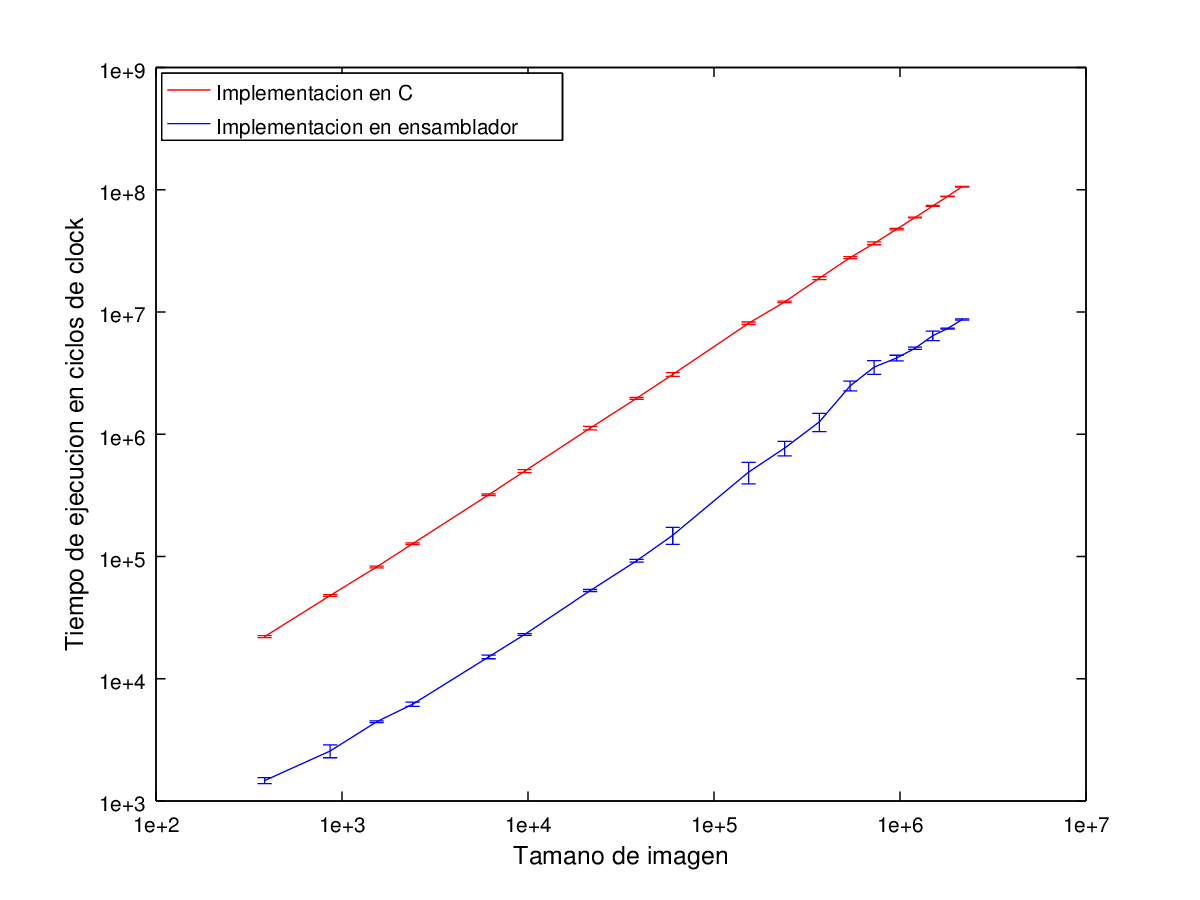
\includegraphics[width=12cm]{../exp/graficos/exp1-diff-c_vs_asm.png} \\
    \end{tabular}}

    {\centering \begin{tabular}{c}
      {\small Filtro Diferencia - Tiempo de ejecución normalizado por píxel} \\
      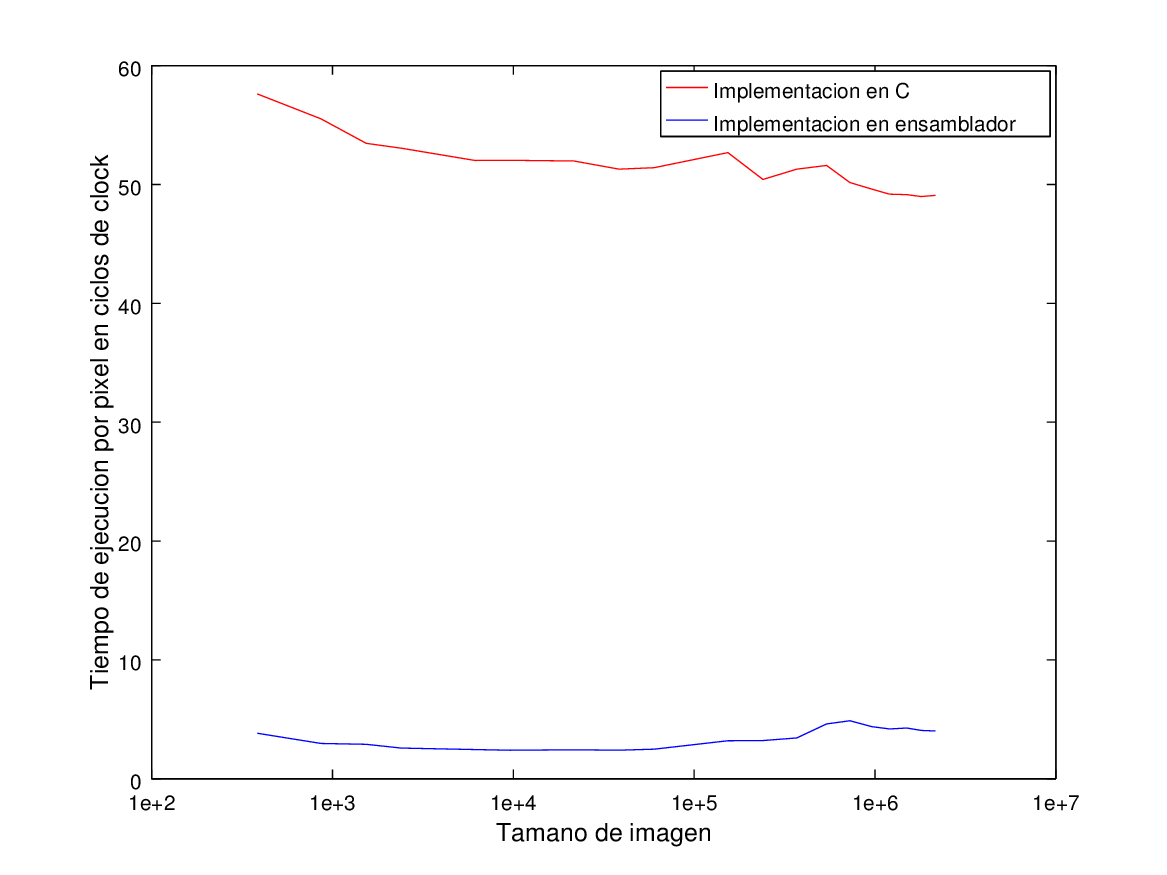
\includegraphics[width=12cm]{../exp/graficos/exp1-diff-tiempo_por_pixel.png} \\
    \end{tabular}}

	{\centering \begin{tabular}{c}
      {\small Filtro Blur} \\
      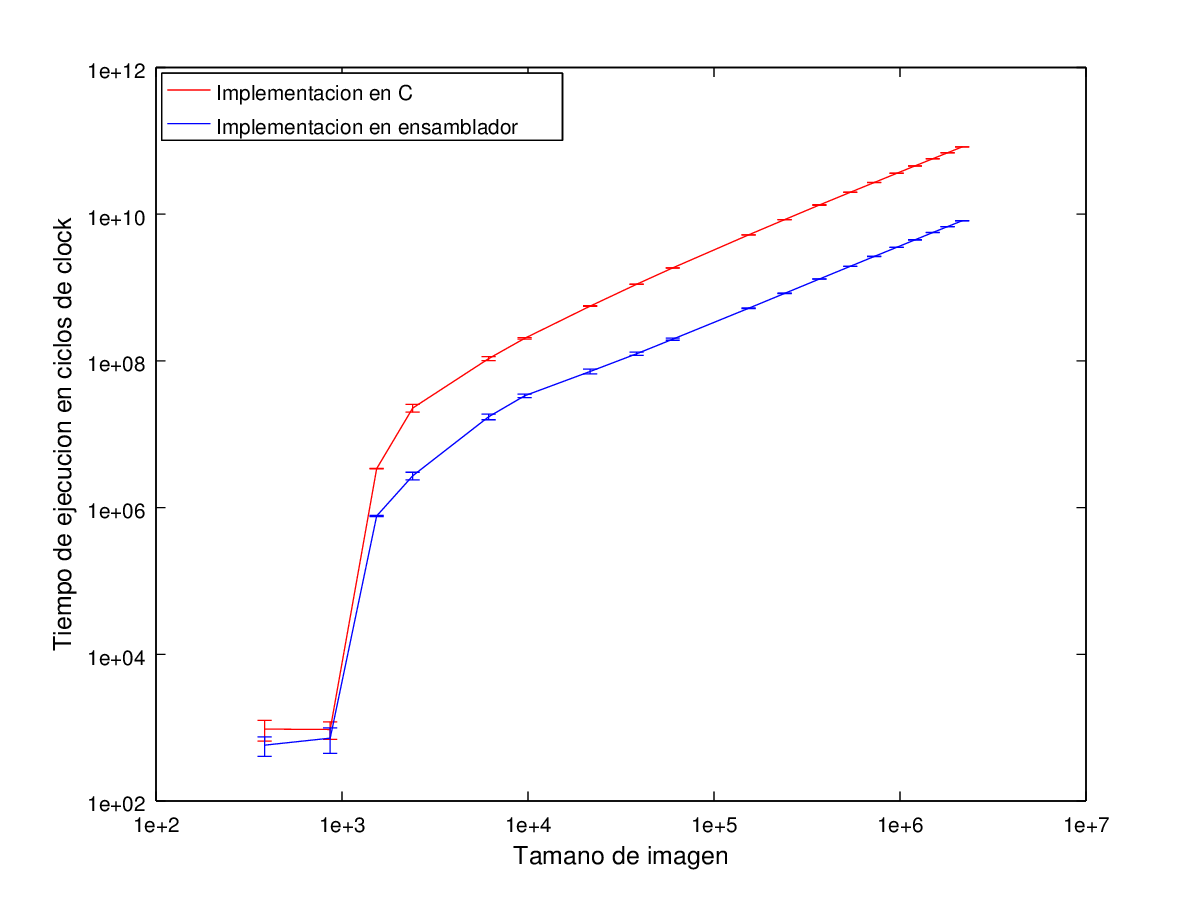
\includegraphics[width=12cm]{../exp/graficos/exp1-blur-c_vs_asm.png} \\
    \end{tabular}}

   	{\centering \begin{tabular}{c}
      {\small Filtro Blur - Tiempo de ejecución normalizado por píxel} \\
      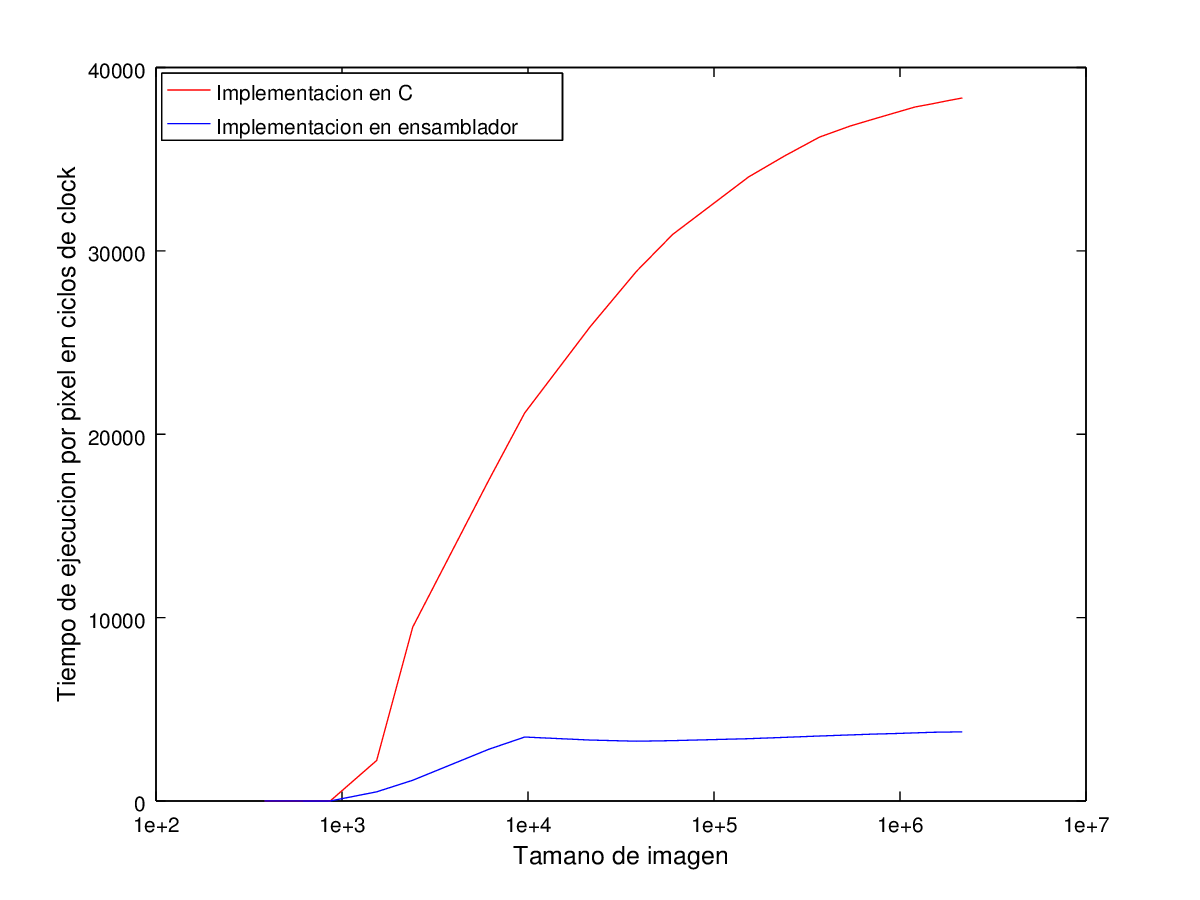
\includegraphics[width=12cm]{../exp/graficos/exp1-blur-tiempo_por_pixel.png} \\
    \end{tabular}}


	\subsubsection{Conclusión} 
		Como se observa en los resultados, la implementación en assembler es más rápida que la implementación en C para todos los tamaños de imagen. Esto se debe a que la primera utiliza SIMD para procesar los píxeles mientras que la segunda no. Lo pudimos comprobar desensamblando el archivo objeto y examinando el código. 


	\subsection{Experimento 2}
		El objetivo de este experimento es observar como se afecta la eficiencia del algoritmo Blur, en cada una de las implementaciones al tomar siempre la misma imagen pero variando el radio.
	
		De esta forma, podemos ver la diferencia de tiempo de ejecución para distintos valores de este parámetro, tanto para la implementación en C como la de assembler. Este experimento lo vamos a realizar normalizando el resultado, para considerar el tiempo de procesamiento por píxel.

		\subsubsection{Hipótesis} 
			Suponemos que a medida que el valor del radio sea mayor, el tiempo de ejecución en las dos implementaciones aumenta. Esto se debe a que el tamaño de la matriz de convolución y de la submatriz imagen es $(2 \times \mathtt{radio} + 1) \times (2 \times \mathtt{radio} + 1) \times 4$. 

		\subsubsection{Valores utilizados como parámetros} 
		La dimensión de la imagen utilizada es 400 filas y 600 columnas. El valor del sigma es 5 y los radios toman valores entre 1 y 40.

		\subsubsection{Resultados}

		{\centering \begin{tabular}{c}
      		{\small Filtro Blur - Tiempo de ejecución según radio} \\
      		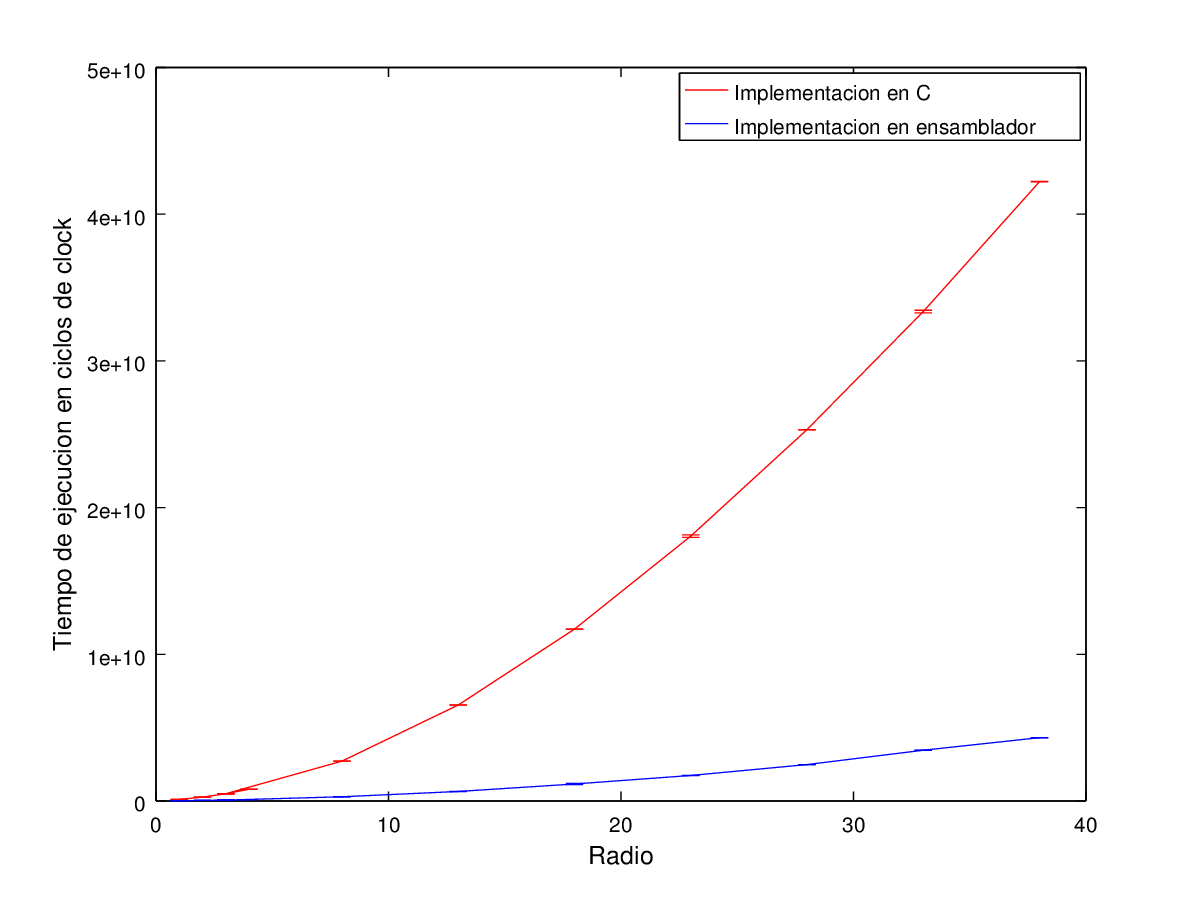
\includegraphics[width=12cm]{../exp/graficos/exp2-tiempo_segun_radio.png} \\
    	\end{tabular}}

		\subsubsection{Conclusión}
			Podemos observar en los gráficos que a medida que los radios aumentan, también lo hace el tiempo de ejecución. Por lo tanto, pudimos comprobar nuestra hipótesis. Esto sucede ya que cuanto mayor es el tamaño de la matriz de convolución, crece la cantidad de iteraciones que se realiza por cada píxel.

			


	\subsection{Experimento 3}
		Este experimento es similar al anterior, también se realiza sobre las dos implementaciones del filtro Blur y se considera siempre la misma imagen. En este caso el radio se mantiene constante pero el valor del sigma se modifica. También se va a utilizar el resultado normalizado, para poder estudiar el tiempo de procesamiento por píxel. 

		\subsubsection{Hipótesis} 
			Debido a que el valor del sigma es utilizado solamente para realizar un cálculo por cada posición de la matriz de convolución, suponemos que modificar este valor no alterará el tiempo de ejecución.

		\subsubsection{Valores utilizados como parámetros} 
		La dimensión de la imagen utilizada es 400 filas y 600 columnas. El valor del radio es 10 y sigma toma valores entre 0.5 y 50.

		\subsubsection{Resultados}

		{\centering \begin{tabular}{c}
      		{\small Filtro Blur - Tiempo de ejecución según sigma} \\
      		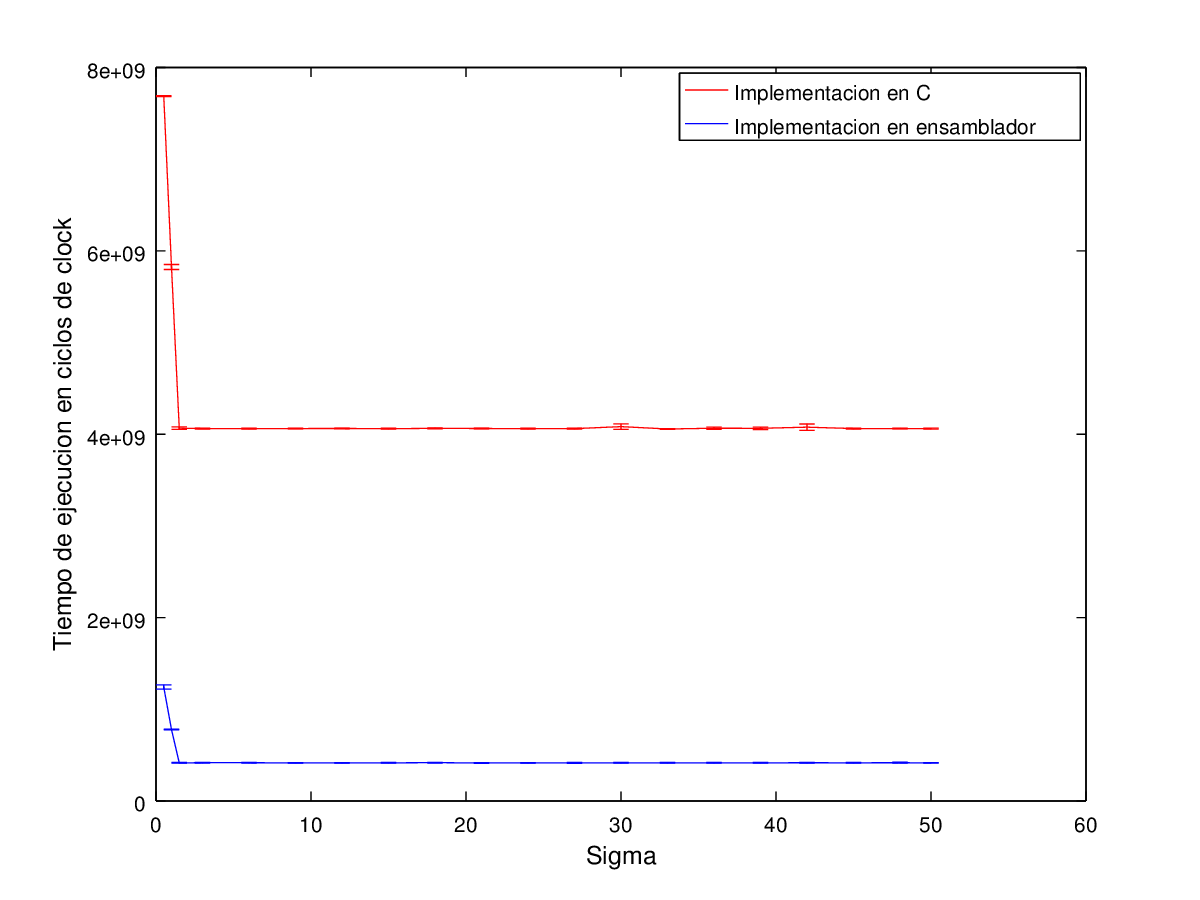
\includegraphics[width=12cm]{../exp/graficos/exp3-tiempo_segun_sigma.png} \\
    	\end{tabular}}

		\subsubsection{Conclusión}


	\subsection{Experimento 4}
		Otras de las pruebas consiste en comparar los tiempos de ejecución de diferentes implementaciones de los filtros en assembler. Nos interesa medir el peso que tienen en el tiempo de ejecución los llamados a funciones auxiliares. Para esto, queremos comparar el rendimiento de una implementación que utiliza llamados a estas funciones, con el de otra que tiene todas las instrucciones necesarias en el mismo bloque de código (sin utilizar esas funciones auxiliares). 
		
		Este experimento se realiza una determinada cantidad de veces con distintos tamaños de imagen.

		\subsubsection{Hipótesis} 
			Creemos que la versión del código implementada en assembler que no realiza llamados a funciones va a tener un mejor rendimiento, ya que se evita el overhead que producen estos llamados.
		
		\subsubsection{Valores utilizados como parámetros} 
			En este experimento el ancho de las imágenes utilizadas como parámetro se encuentran en un rango entre 24 y 1800 píxeles.Además, para el filtro Blur se utilizó $Radio = 15$ y $Sigma = 5$.


		\subsubsection{Resultados}
		{\centering \begin{tabular}{c}
      		{\small Filtro Diferencia} \\
      		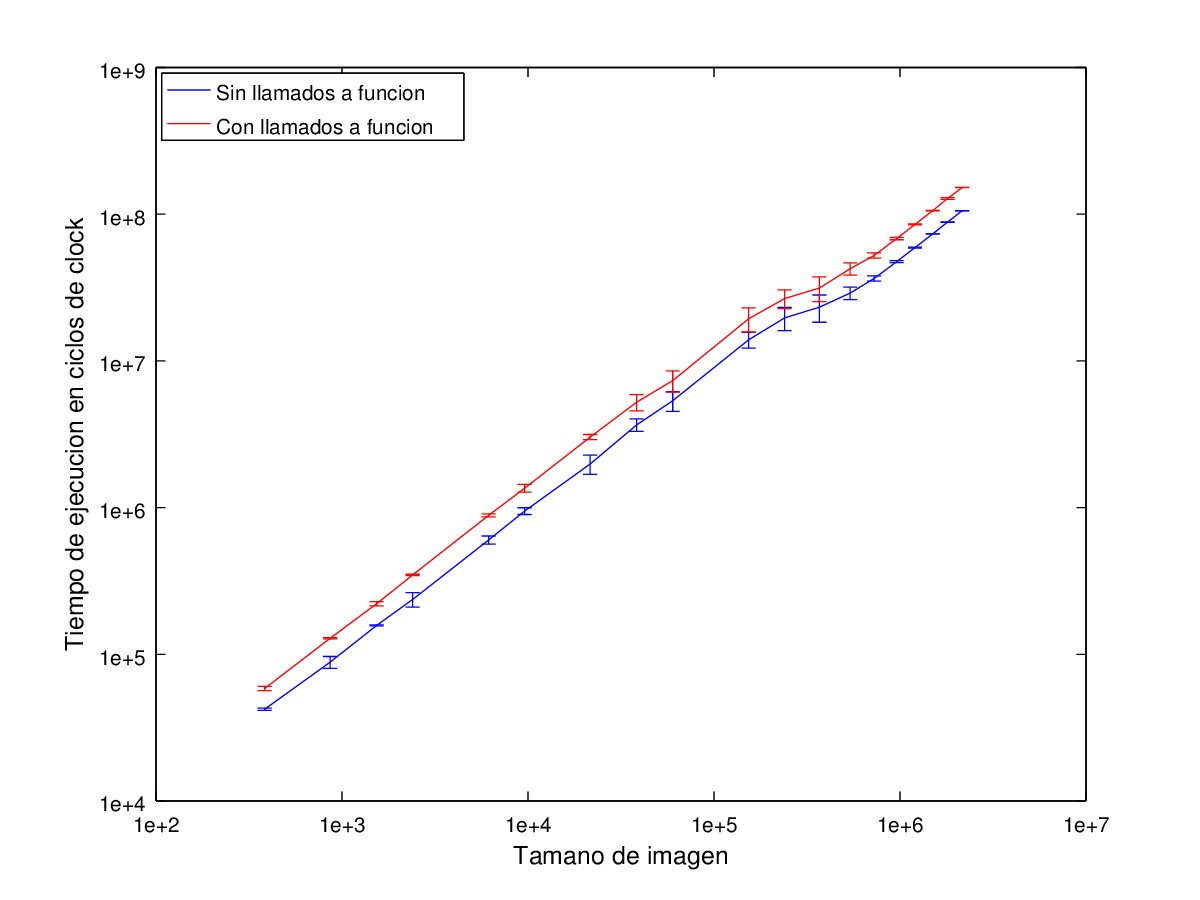
\includegraphics[width=12cm]{../exp/graficos/exp4-diff-c_vs_c2.png} \\
    	\end{tabular}}

		{\centering \begin{tabular}{c}
      		{\small Filtro Blur} \\
      		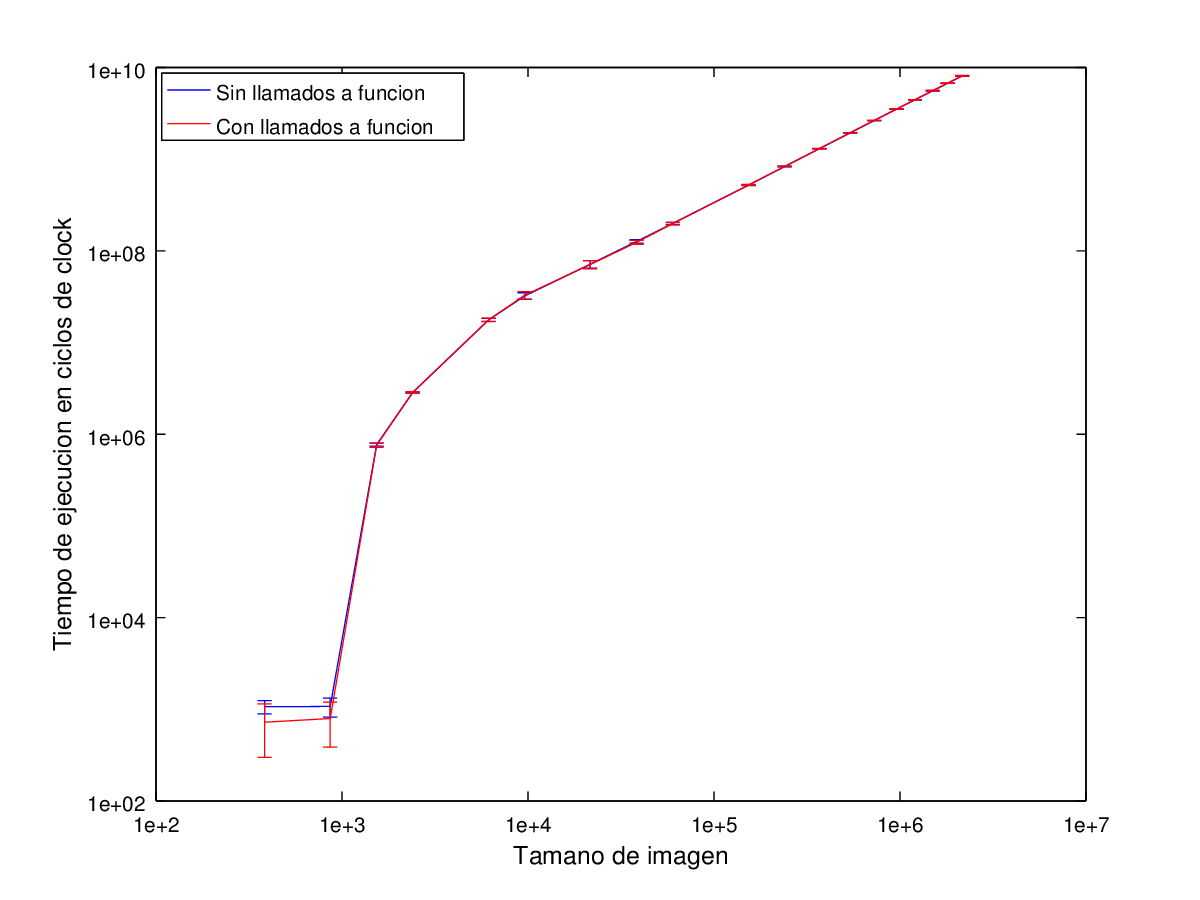
\includegraphics[width=12cm]{../exp/graficos/exp4-blur-asm_vs_asm2.png} \\
    	\end{tabular}}

		\subsubsection{Conclusión}		
\section{Conclusiones}

\clearpage

% Apéndices
% \input{apendices}
% \clearpage

% Referencias
% \printbibliography[heading=bibintoc]

\end{document}
